\makeheading{Lecture 5 | 2020-09-20}
\begin{Example}{Uniqueness Theorem}{}
    Suppose $ M_X(t)=(1-2t)^{-1} $. What is the
    distribution of $ X $?

    \textbf{Solution.} $ X \sim \gam{\alpha=1,\beta=2}$.
\end{Example}

\chapter{Multivariate Random Variables}
\section{Joint and Marginal Cumulative Distribution Functions}
Purpose: to characterize a joint distribution
of two random variables.
\begin{Definition}{Joint cumulative distribution function}{}
    Suppose $ X $ and $ Y $ are random variables defined on
    a sample space $ S $. The \textbf{joint cumulative
        distribution function} of $ X $ and $ Y $ is given by
    \[ F(x,y)=\Prob{X\le x,Y\le y} \]
    for $ (x,y)\in\mathbb{R}^2 $.
\end{Definition}
$ \Prob{X\le x,Y\le y} $:
``What is the probability these two events occur simultaneously''
\begin{Remark}{}{}
    Since $ \set{X\le x} $ and $ \set{Y\le y} $
    are both events, $ F(x,y) $ is well-defined as
    we consider $ \set{X\le x}\cap \set{Y\le y} $.
\end{Remark}
\begin{Remark}{}{}
    If we have more than two random variables, say $ X_1,X_2,\ldots,X_n $
    We can similarly define the cumulative distribution function as
    \[ F(x_1,\ldots,x_n)=\Prob{X_1\le x_1,\ldots,X_n\le x_n} \]
    However, in this course we will only focus on two events $ X $ and $ Y $.
\end{Remark}

\begin{Definition}{Joint cumulative distribution function}{}
    \begin{enumerate}[label=(\Roman*)]
        \item $ F $ is non-decreasing in $ x $ for fixed $ y $
        \item $ F $ is non-decreasing in $ y $ for fixed $ x $
        \item $ \displaystyle \lim\limits_{{x} \to {-\infty}} F(x,y)=0 $
              and $ \displaystyle \lim\limits_{{y} \to {-\infty}} F(x,y)=0 $

              By looking at
              \[ \underset{\underset{\text{ as }x\to-\infty}{\to 0}}{\set{X\le x}}\cap
                  \underset{\underset{\text{ as }y\to-\infty}{\to 0}}{\set{Y\le y}} \]
        \item \[ \displaystyle
                  \smashoperator{\lim\limits_{{(x,y)} \to {(-\infty,-\infty)}}}
                  F(x,y)=0\text{ and }
                  \displaystyle
                  \smashoperator{\lim\limits_{{(x,y)} \to {(\infty,\infty)}}}
                  F(x,y)=1 \]
    \end{enumerate}
\end{Definition}

\begin{Definition}{Marginal distribution function}{mdf}
    The \textbf{marginal distribution function} of $ X $ is given by
    \[ F_1(x)=\lim\limits_{{y} \to {\infty}} F(x,y)=\Prob{X\le x} \]
    for $ x\in\mathbb{R} $.

    The \textbf{marginal distribution function} if $ Y $ is given by
    \[ F_2(y)=\lim\limits_{{x} \to {\infty}} F(x,y)=\Prob{Y\le y} \]
    for $ y\in\mathbb{R} $.
\end{Definition}
\begin{Remark}{}{}
    The definition of marginal distribution
    function tells us that we can know all information
    about marginal c.d.f.\ from the joint c.d.f.\ but the
    marginal c.d.f.\ cannot give full information about
    joint c.d.f.\
\end{Remark}
\section{Bivariate Discrete Distributions}
\begin{Definition}{Joint discrete random variables}{}
    Suppose $ X $ and $ Y $ are both discrete random variables,
    then $ X $ and $ Y $ are \textbf{joint discrete random variables}
    $ X $ and $ Y $.
\end{Definition}

\begin{Definition}{Joint probability function, Support set}{}
    Suppose $ X $ and $ Y $ are discrete random variables.
    The \textbf{joint probability function} of $ X $ and $ Y $
    is given by
    \[ f(x,y)=\Prob{X=x,Y=y} \]
    for $ (x,y)\in\mathbb{R}^2 $.

    The set $ A=\left\{ (x,y):f(x,y)>0 \right\} $ is called
    the \textbf{support set} of $ (X,Y) $.
\end{Definition}

\begin{Definition}{Properties --- Joint Probability Function}{}
    \begin{enumerate}[label=(\Roman*)]
        \item $ f(x,y)\ge 0 $ for $ (x,y)\in\mathbb{R}^2 $
        \item $ \displaystyle \sum\limits_{(x,y)\in A}
                  f(x,y)=1 $
        \item For any set $ R\subseteq \mathbb{R}^2 $
              \[ P\left[ (X,Y)\in R \right]
                  =\sum\limits_{(x,y)\in R}f(x,y)  \]
    \end{enumerate}
\end{Definition}

\begin{Example}{}{}
    Suppose we want to find $ \Prob{X\le Y} $. What is the
    corresponding set $ R $?

    \textbf{Solution.} $ R=\set{(x,y):x\le y} $

    Suppose we want to find $ \Prob{X+Y\le 1} $. What is the corresponding
    set $ R $?

    \textbf{Solution.} $ R=\set{(x,y):x+y\le 1} $
\end{Example}

\begin{Definition}{Marginal probability function}{}
    Suppose $ X $ and $ Y $ are discrete
    random variables with joint probability
    function $ f(x,y) $.

    The \textbf{marginal probability
        function} of $ X $ is given by
    \[ f_1(x)=\Prob{X=x}
        =\Prob{X=x,Y<\infty}
        =\sum\limits_{y}f(x,y)  \]
    for $ x\in\mathbb{R} $.

    The \textbf{marginal probability function} of $ Y $
    is given by
    \[ f_2(y)=\Prob{Y=y}
        =\Prob{X<\infty,Y=y}
        =\sum\limits_{x}f(x,y)  \]
    for $ y\in\mathbb{R} $.
\end{Definition}

\begin{Example}{}{}
    Suppose that $ X $ and $ Y $ are discrete random variables
    with joint p.f.\ $ f(x,y)=kq^2 p^{x+y} $ where
    \begin{itemize}
        \item $ x=0,1,2,\ldots $
        \item $ y=0,1,2,\ldots $
        \item $ 0<p<1 $
        \item $ q=1-p $
    \end{itemize}
    \begin{enumerate}[label=(\roman*)]
        \item Determine $ k $.
        \item Find marginal p.f.\ of $ X $ and
              find marginal p.f.\ of $ Y $.
        \item Find $ \Prob{X\le Y} $.
    \end{enumerate}
    \textbf{Solution.}
    \begin{enumerate}[label=(\roman*)]
        \item $ k>0 $ since if $ k=0 $ then the summation
              of the joint p.f.\ will be 0 (but needs to be 1).
              \[\sum\limits_{x=0}^{\infty}
                  \sum\limits_{y=0}^{\infty} f(x,y)=1\]
              Therefore,
              \[k\biggl(\sum\limits_{x=0}^{\infty}
                  \sum\limits_{y=0}^{\infty} p^{x+y}q^2\biggr)=
                  kq^2\biggl(\sum\limits_{x=0}^{\infty} p^x\biggr)
                  \biggl(\sum\limits_{y=0}^{\infty}p^y\biggr)=kq^2
                  \left( \frac{1}{1-p}  \right)\left( \frac{1}{1-p} \right)=k
              \]
              Thus, $ k=1 $.
        \item Marginal p.f.\ of $ X $:
              \[ f_1(x)=\Prob{X=x}=
                  \sum\limits_{y=0}^{\infty} q^2p^{x+y}=
                  q^2 p^x
                  \biggl(\sum\limits_{y=0}^{\infty} p^y \biggr)
                  =q^2 p^x \left( \frac{1}{1-p}  \right)=p^x(1-p) \]
              Support of $ X $: $ x=0,1,2,\ldots $.

              By symmetry,
              \[ f_2(y)=\Prob{Y=y}=qp^y \]
              Support of $ Y $: $ y=0,1,2,\ldots $.
        \item Find $ \Prob{X\le Y} $.

              \begin{align*}
                  \Prob{X\le Y}
                   & =
                  \sum\limits_{x=0}^{\infty}
                  \sum\limits_{y=x}^{\infty}\left( q^2 p^{x+y} \right) \\
                   & =\sum\limits_{x=0}^{\infty} q^2p^x
                  \sum\limits_{y=x}^{\infty} p^y                       \\
                   & =\sum\limits_{x=0}^{\infty}
                  q^2p^x\left( \frac{p^x}{1-p}  \right)                \\
                   & =q\sum\limits_{x=0}^{\infty} p^{2x}               \\
                   & =q\left( \frac{1}{1-p^2}  \right)                 \\
                   & =\frac{1}{1+p}
              \end{align*}

    \end{enumerate}
\end{Example}
\begin{Remark}{Interesting Fact}{}
    If $ X $ and $ Y $ are \emph{continuous} random variables
    and have the same distribution and \emph{\textbf{independent}},
    \[ \Prob{X\le Y}=\frac{1}{2} \]
\end{Remark}
\section{Bivariate Continuous Distributions}
\begin{Definition}{Joint probability density function, Support set}{}
    Suppose that $ F(x,y) $ is a continuous
    function and that
    \[ f(x,y)=\frac{\partial^2}{\partial x\partial y}\left[ F(x,y) \right]  \]
    exists and is a continuous function
    except possibly along a finite number of curves.
    Suppose also that
    \[ \int_{-\infty}^{\infty} \int_{-\infty}^{\infty} f(x,y)\, d{x}\, d{y}=1  \]
    Then $ X $ and $ Y $ are said to be continuous random
    variables with \textbf{joint probability density function} $ f $.

    The set $ A=\set{(x,y):f(x,y)>0} $ is called the support set of $ (X,Y) $.
\end{Definition}
\begin{Remark}{}{}
    We will arbitrarily define $ f(x,y) $ to be equal to $ 0 $ when
    $ \displaystyle  \frac{\partial^2}{\partial x\partial y}\left[ F(x,y) \right]
    $
    does not exist, although we can define it to be any real number.
\end{Remark}
\begin{Definition}{Properties --- Joint Probability Density Function}{}
    \begin{enumerate}[label=(\Roman*)]
        \item $ f(x,y)\ge 0 $ for all $ (x,y)\in\mathbb{R}^2 $
        \item For any set $ R\subseteq \mathbb{R}^2 $:
              \begin{align*}
                  P\left[ (X,Y)\in R \right]
                   & =\iint\limits_{(x,y)\in R}f(x,y)dx\,dy
              \end{align*}
    \end{enumerate}
\end{Definition}
\begin{Example}{}{}
    To find $ \Prob{X\le Y} $, the region is
    $ R=\set{(x,y):x\le y} $. Therefore,
    \[ \Prob{X\le y}=
        \iint\limits_{x\le y}f(x,y)dx\,dy \]
\end{Example}
\begin{Definition}{Marginal probability density function}{}
    Suppose $ X $ and $ Y $ are continuous random variables with
    p.d.f.\ $ f(x,y) $. The \textbf{marginal probability
        density function} of $ X $ is given by
    \[ f_1(x)=\int_{-\infty}^{\infty} f(x,y)\, d{y} \]
    for $ x\in\mathbb{R} $ and the \textbf{marginal probability
        density function} of $ Y $ is given by
    \[ f_2(y)=\int_{-\infty}^{\infty} f(x,y)\, d{x}  \]
    for $ y\in\mathbb{R} $.
\end{Definition}
\[ P\left[ (X,Y)\in\mathbb{R} \right]
    =\iint\limits_{R}f(x,y)dx\,dy=
    \int_{x} \int_{y}f(x,y) \, d{x} \, d{y} \]
Helpful theorem from MATH 237 that some of you may have forgot:

\begin{Theorem}{$ \dagger $}{}
    \underline{$ y $ first, then $ x $}

    Let $ R\subset \mathbb{R}^2 $ be defined by
    \[ y_\ell(x)\le y\le y_u(x)\quad\text{ and }\quad
        x_{\ell}\le x\le x_u \]
    where $ y_{\ell}(x) $ and $ y_u(x) $ are continuous
    for $ x_{\ell}\le x\le x_u $. If $ f(x,y) $
    is continuous on $ R $, then
    \[ \iint\limits_{R}f(x,y)dA=
        \int_{x_\ell}^{x_u} \int_{y_\ell(x)}^{y_u(x)} f(x,y)\, d{y} \, d{x}  \]
    \underline{$ x $ first, then $ y $}

    Let $ R\subset \mathbb{R}^2 $ be defined by
    \[ x_\ell(y)\le x\le x_u(y)\quad\text{ and }\quad
        y_{\ell}\le y\le y_u \]
    where $ x_{\ell}(y) $ and $ x_u(y) $ are continuous
    for $ y_{\ell}\le y\le y_u $. If $ f(x,y) $
    is continuous on $ R $, then
    \[ \iint\limits_{R}f(x,y)dA=
        \int_{y_\ell}^{y_u} \int_{x_\ell(y)}^{x_u(y)} f(x,y)\, d{x} \, d{y}  \]
\end{Theorem}
We use $ \ell $ for ``lower'' amd $ u $ for ``upper.''
\begin{Example}{}{}
    Describe the region $ R $ above the $ x $-axis.
    \begin{center}
        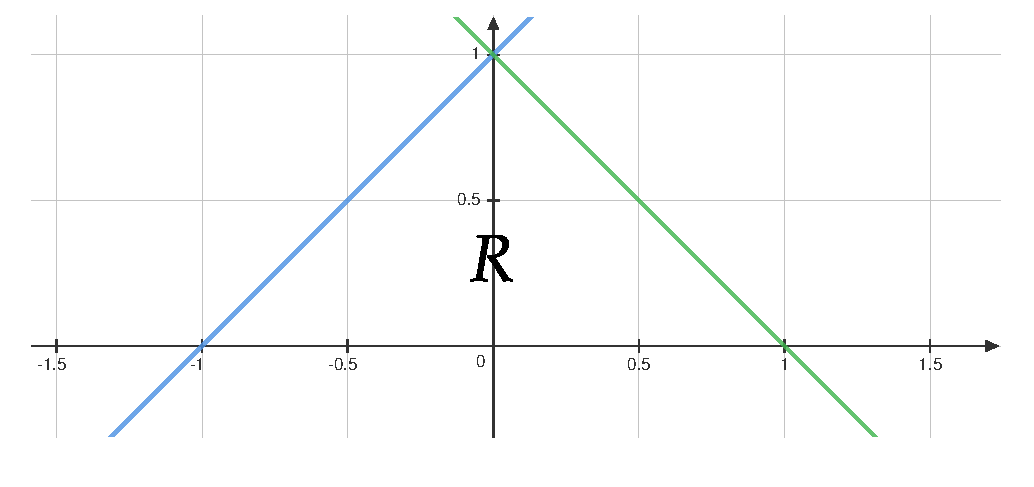
\includegraphics[width=0.9\textwidth]{fig1.pdf}
    \end{center}
    \textbf{Solution.} $ R $ can be described by the set of two inequalities
    (you can actually verify this in Desmos if you \emph{really} forgot how this works):
    \[ 0\le y\le 1 \]
    \[ y-1\le x\le 1-y \]
    Using the theorem above,
    \[ \int_{0}^{1} \int_{y-1}^{1-y} f(x,y)\, d{x}\, d{y}  \]
\end{Example}
